\documentclass[a4paper,10pt]{article} 	% A4 papir, 10pt størrelse
\usepackage[english]{babel}
\usepackage{Nikolai} 					% Min hjemmelavede pakke
\usepackage[dvipsnames]{xcolor}

% Margen
\usepackage[margin=1in]{geometry}

% Max antal kolonner i en matrix. Default er 10
%\setcounter{MaxMatrixCols}{20}

% Hvor dybt skal kapitler labeles?
%\setcounter{secnumdepth}{4}	
%\setcounter{tocdepth}{4}


% Hvilket nummer skal der startes med i sections? (n-1)
%\setcounter{section}{0}	

% Til nummerering af ligninger. Så der står (afsnit.ligning) og ikke bare (ligning)
\numberwithin{equation}{section}


% Header
%\usepackage{fancyhdr}
%\head{}
%\pagestyle{fancy}

%Titel
\title{Numerical Methods in Physics Week 3}
\author{Nikolai Plambech Nielsen}
\date{}

\begin{document}
	\maketitle
	\section{Prisoners dilemma}
	The prisoners dilemma game is a common though experiment in game theory in which cooperation is studied. In its most basic form it consists of two participants, who are both imprisoned. They have the choice of cooperating or cheating (from here-on called deferring) in a game. If they both choose to cooperate, their sentences are reduced by 1 unit of time (say, a year), if one of them defers, then the deferrers sentence is reduced by $ b $ units of time (usually more than 1), whilst the cooperators sentence is not reduced by any amount. If they both defer, neither of their sentences are reduced.
	
	So the optimal outcome for the individual is to cheat and the other to cooperate, as this has the highest payoff. But if $ b $ is between 1 and 2, then cooperation reduces the overall sentences by more than just one person cheating. Of course, cheating is a gamble, as if both participants do this, neither get any payoff.
	
	For this assignment, the prisoners dilemma game is expanded to be played on a square, two dimensional lattice of size $ n $-by-$ n $, and in every round, every participant plays the game with each of its 8 neighbours (and itself, for ease of programming). The payoff of each of these 9 individual games are recorded in a matrix, after which every participant checks all 8 neighbours and itself for the highest payoff and adopts the strategy of this participant. This process is then repeated for a specified amount of iterations, with different initial conditions (the value of $ b $, the initial starting strategies, etc).
	
	There are also the question of boundary conditions. For the simplicity of programming, cyclic boundary conditions are chosen such that the lattice wraps around itself at all four sides. 
	
	To make changes in strategy clearer, four colours are used, depending on the strategies of the individuals in the current and previous round. If an individual currently cooperates, and cooperated before, it is blue. If it deferred before, it is green. If the individual currently defers, and deferred before, it is red. But if it cooperated before, it is yellow. Below is shown an example where $ b = 1.85, n=75 $, and where all starting strategies are to cooperate, except for the middle individual (38th row and column), who defers.
	
	\begin{figure}[H]
		\centering
		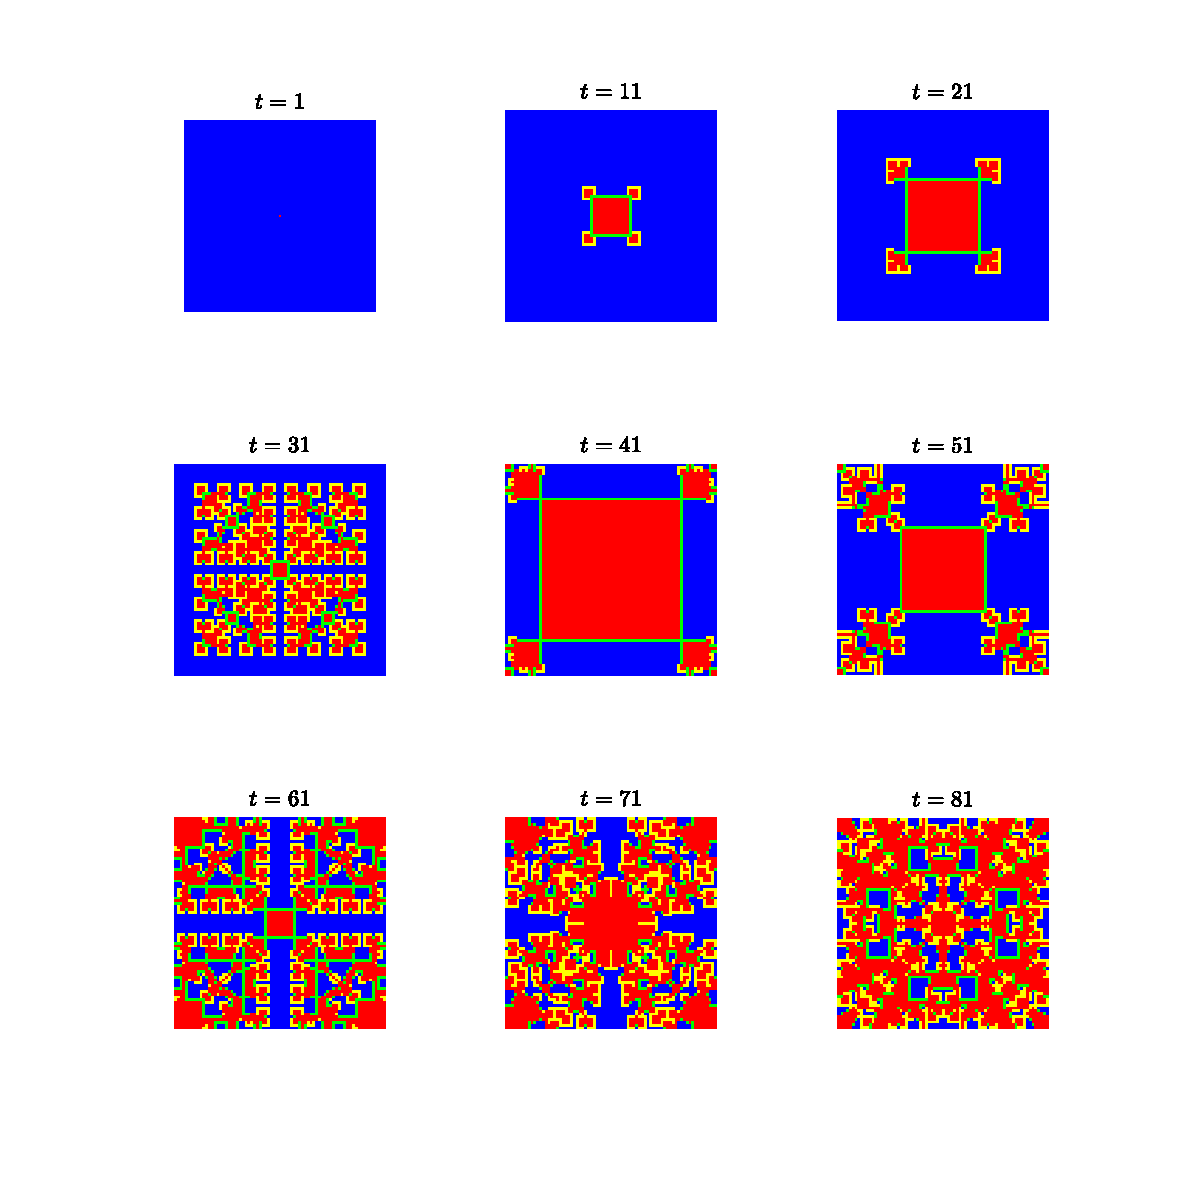
\includegraphics[width=\linewidth]{prisonersnapshot1}
		\caption{9 snapshots of the prisoners dilemma game, for $ b=1.85, n=75 $, where the starting configuration is all but the middle individual cooperating.}
		\label{fig:prisonersnap}
	\end{figure}
	
	While the shapes are symmetrical, there seems to be no temporal pattern or repetition present. This is checked for $ 5\D 10^5 $ iterations, where the strategies are checked (not the colours, making for a less stringent condition) with all previous strategies. However, if the number of individuals with a given colour is plotted, the count does seem to gravitate towards some form of mean. While this is certainly not an equilibrium of any sort (at least for the first $ 5\D 10^5 $ iterations), there does seem to be a sort of order to the number of individuals for a given colour:
	
	\begin{figure}[H]
		\centering
		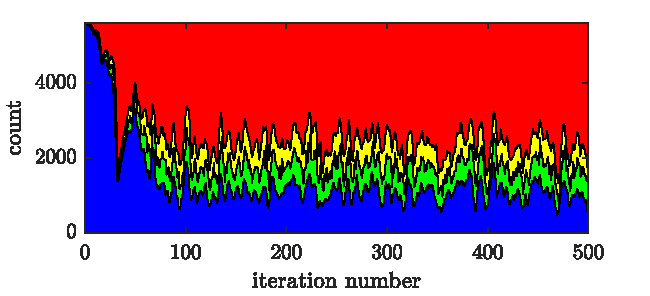
\includegraphics[width = 0.75\linewidth]{prisonercount1}
		\caption{The number of individuals with a given colour, for the initial conditions of the previous figure. There are no repetition in the strategies, but the count of individuals do seem to fluctuate around a mean}
		\label{fig:prisonercount1}
	\end{figure}

	This is not to say that equilibria do not form. For the same initial starting strategies, if $ 1.6 \leq b < 1.8 $, a static equilibrium is quickly established, where the middle 9 individuals all defer, but the rest cooperate. For $ 1.25 < b < 1.6 $ a dynamic equilibrium is encountered, where the middle individual is always deferring, but its 8 neighbours either all defer or all cooperate, changing with each iteration. The "pattern" occurring for $ b=1.85 $ happens for all $ 1.8<b<2 $.
	
	One may wonder why these "ranges" appear. This is because the payoffs is only in multiples of 1 or $ b $, so the pattern only changes, when points of the form $ n=mb $, for constant integers $ n,m $ are passed. Values of $ b $ where the equality $ n=mb $ holds give insight into the programming of the game. At these values, there might be neighbours with the same payoff but different strategies. The outcomes then depend on how these cases are handled. In my program, the comparing of payoffs follows the layout of a phone keypad: the top left neighbour, down to the bottom right. If the top left and bottom right both have the highest payoff but different strategies, then the middle individual will chose the top left strategy. This is easily seen for $ b=1.8 $:
	
	\begin{figure}[H]
		\centering
		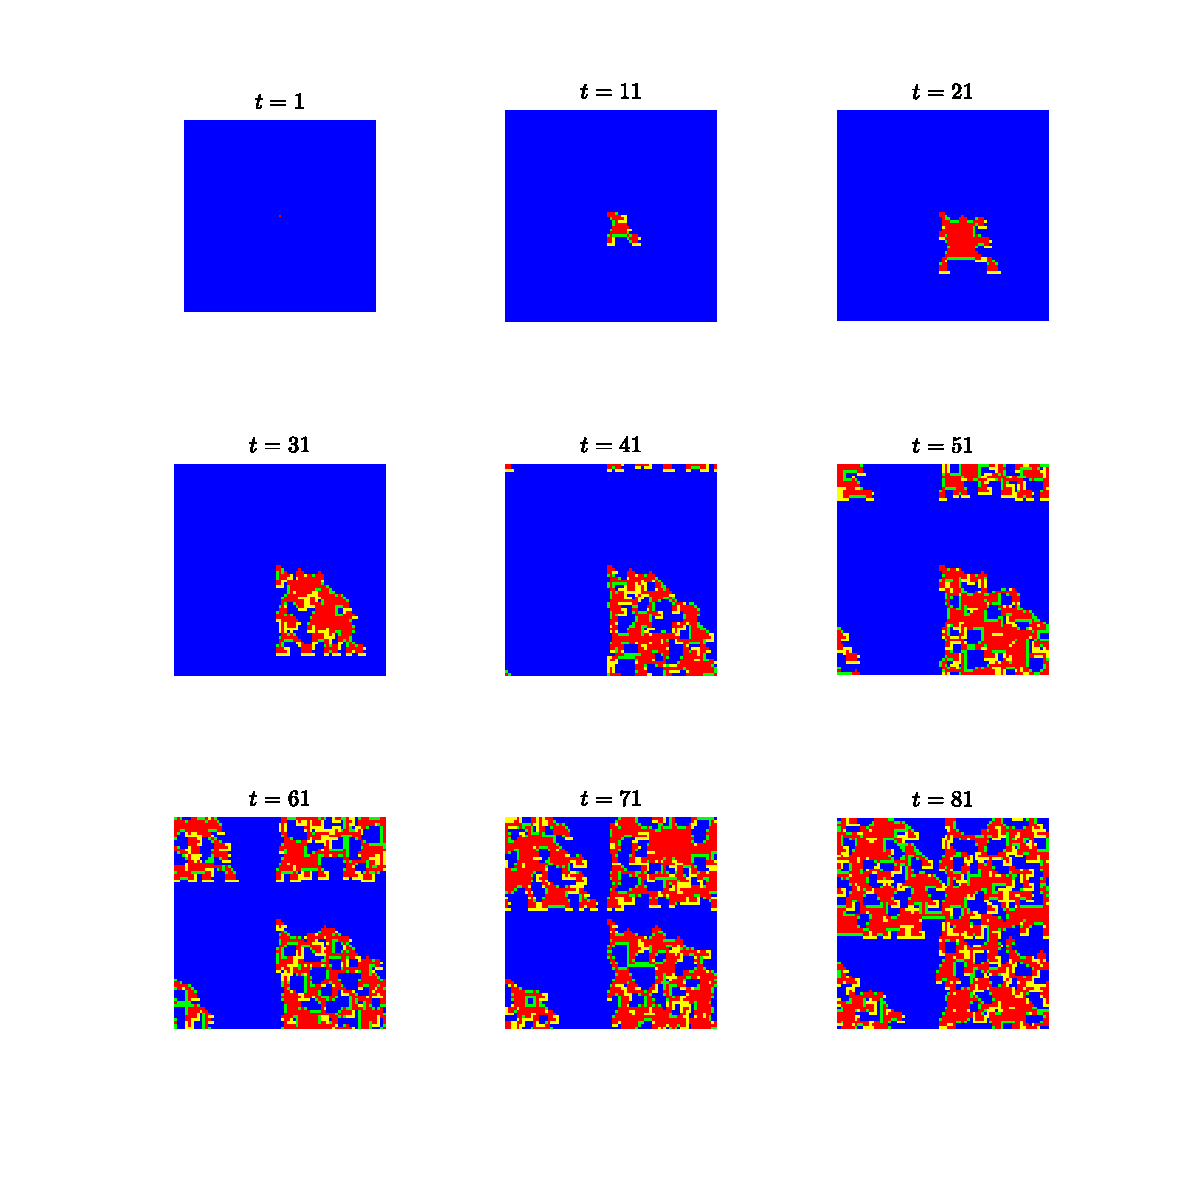
\includegraphics[width=\linewidth]{prisonersnapshot2}
		\caption{9 snapshots for $ b=1.8 $. The bias towards the top left neighbours strategy is evident, as the deferring is spreading down and to the right.}
		\label{fig:snapshot2}
	\end{figure}


	As one might expect, there is also no repetition when starting with random strategies. There do however seem to be smaller fluctuations in the number of individual with a given colour:
	\begin{figure}[H]
		\centering
		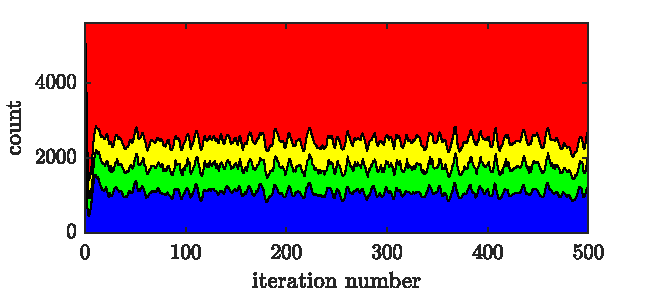
\includegraphics[width=0.75\linewidth]{prisonercountRand}
		\caption{The number of individuals with a given color for random starting strategies. $ b = 1.85 $.}
		\label{fig:countRand}
	\end{figure}
	The mean values and standard deviation (rounded to the neares integer) of the different colours for this random start, and for the start with just one deferring individual are as follows
	\begin{table}[H]
		\centering
		\begin{tabular}{c|c|c}
			Color & Random start & Non-random start \\
			\hline
			Blue 	& $ 1095 \pm 219 $	& $ 1424 \pm 981 $\\
			Green 	& $ 689 \pm 134 $	& $ 601 \pm 236 $\\
			Yellow 	& $ 683 \pm 68 $	& $ 592 \pm 202 $\\
			Red 	& $ 3158 \pm 235 $	& $ 3008 \pm 762 $
		\end{tabular}
	\end{table}
	And yes, the random start does have smaller standard deviations for every colour. My guess for this is that the randomness plays out in such a way as to "dissuade" a lot of fluctuations away from the mean, whilst this is not the case for the non-random start.

	
	\section{Network Percolation}
	In this assignment, the effects of removing nodes from a network are explored. The size of the largest cluster in a network is plotted, as the nodes with the most connections are removed from the network (if there are multiple nodes with the same number of connections, the one with the lowest id is chosen), along with removing random nodes. For a random network of 1000 nodes, with an average of 6.456 connections the result is:
	
	\begin{figure}[H]
		\centering
		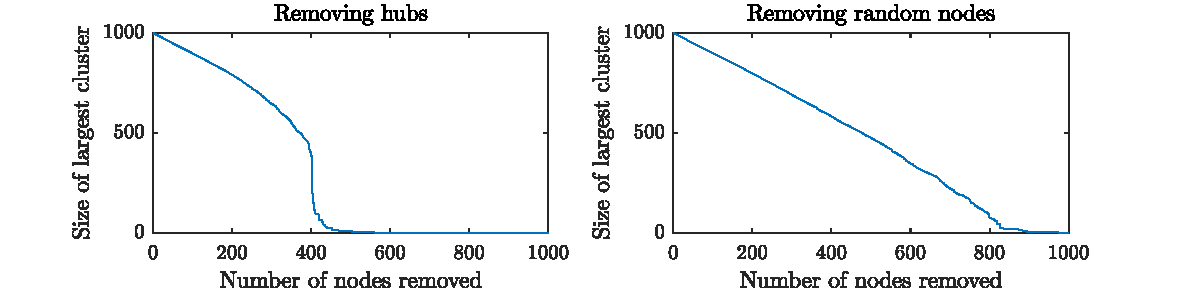
\includegraphics[width=\linewidth]{NetworkRandom}
		\caption{Percolation on a random network of 1000 nodes, with an average of $ 6.456 \pm 2.446 $ connections.}
		\label{fig:networkRand}
	\end{figure}
	The random removal of nodes looks as expected, but the removal of hubs does not. There is a sharp drop-off but it does not happen instantly.
	
	The same is seen for real life networks (all of the examples below are from \url{http://deim.urv.cat/~aarenas/data/welcome.htm}), like the email network at Universitat Rovira i Virgili:
	\begin{figure}[H]
		\centering
		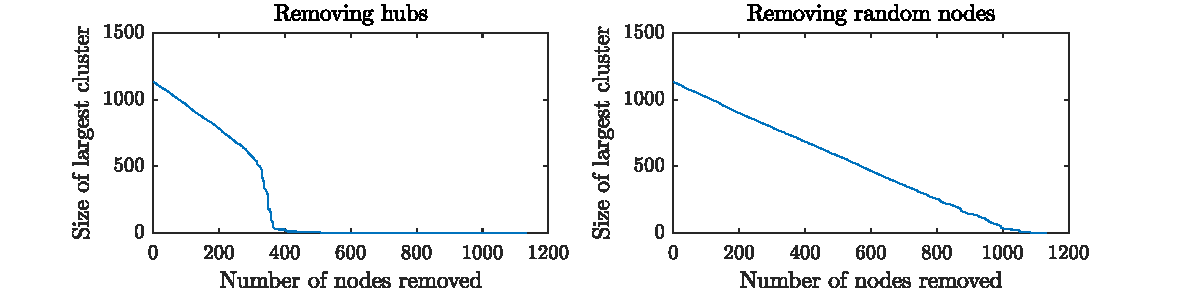
\includegraphics[width=\linewidth]{NetworkEmail}
		\caption{Percolation on an email network at URV.}
		\label{fig:networkEmail}
	\end{figure}
	a network of jazz musicians:
	\begin{figure}[H]
		\centering
		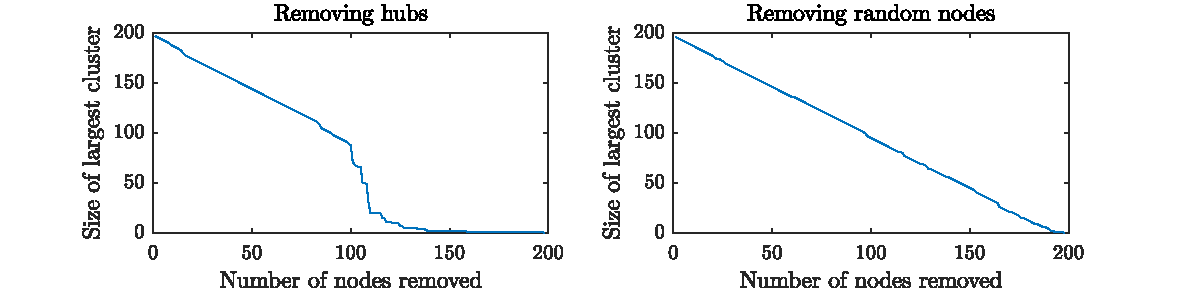
\includegraphics[width=\linewidth]{NetworkJazz}
		\caption{Percolation on a network of jazz musicians.}
		\label{fig:networkJazz}
	\end{figure}
	the metabolic network of C. elegans:
	\begin{figure}[H]
		\centering
		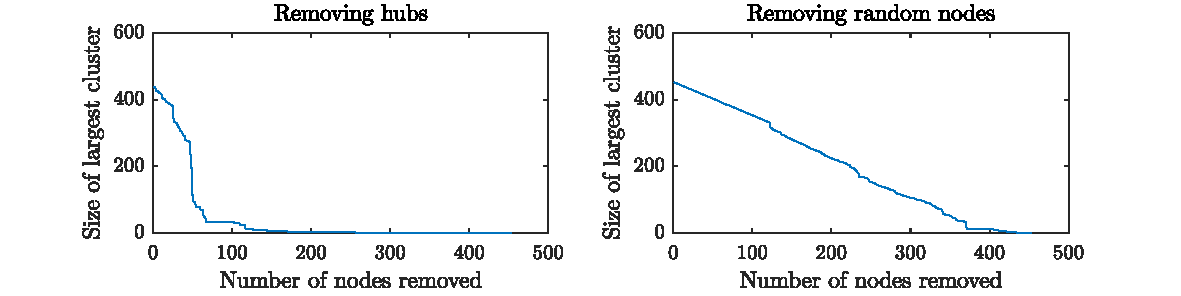
\includegraphics[width=\linewidth]{NetworkMeta}
		\caption{Percolation on the metabolic network for C. elegans.}
		\label{fig:networkMeta}
	\end{figure}
	
	Lastly the removal of hubs is performed on a component of the network for users of the PGP algorithm:
	\begin{figure}[H]
		\centering
		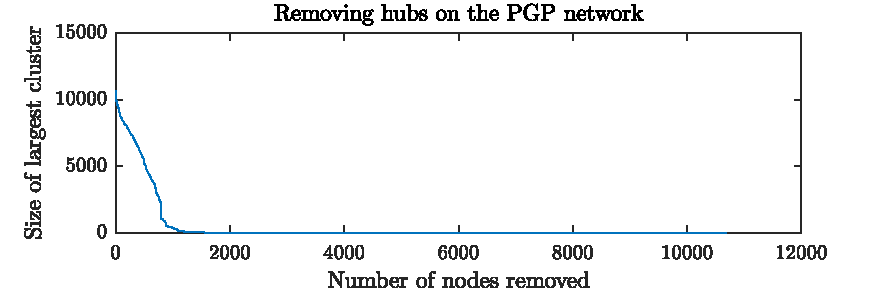
\includegraphics[width=0.7\linewidth]{NetworkPGP}
		\caption{Percolation on a network of PGP users.}
		\label{fig:networkPGP}
	\end{figure}
	Again sharp drop-offs are seen for the removal of hubs, but for the email and jazz musician networks, there is a period of almost linear decrease in cluster size. This is most likely due to a larger number of highly interconnected hubs in the first two networks. A look at the histograms of the number of connections for the four networks does show a larger drop-off for the metabolic and PGP networks:
	\begin{figure}[H]
		\centering
		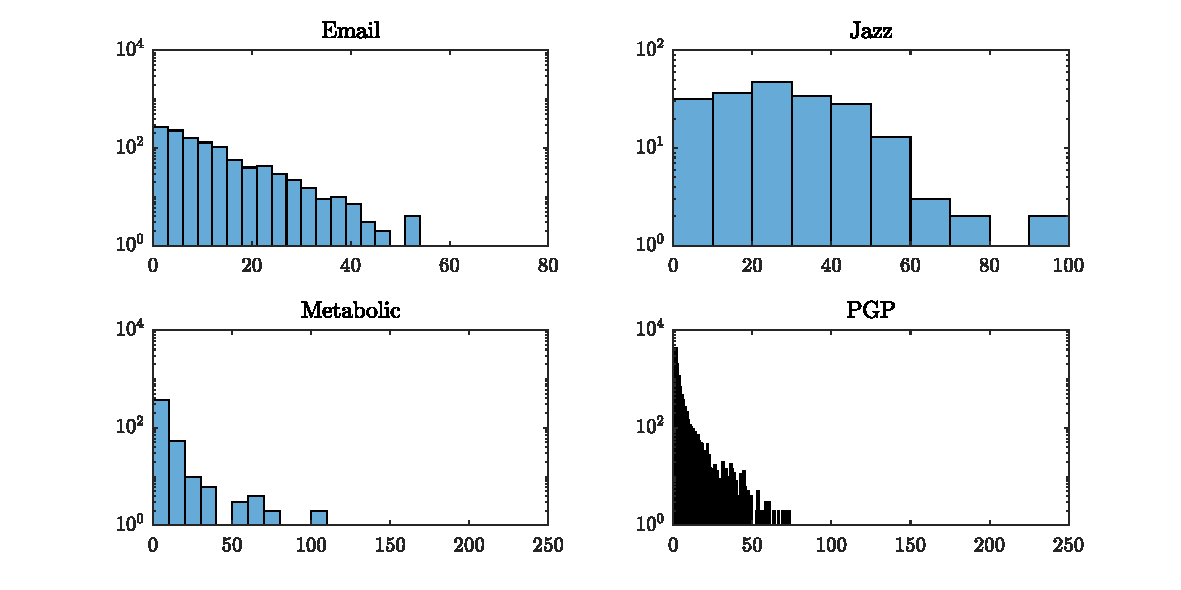
\includegraphics[width=0.7\linewidth]{Hists}
		\caption{Histograms of the number of connections in the four real life networks. Note the log scale on the number of connections. The largest number of connections on the PGP network is 205, but this is for some reason not visible on the histogram when using log-scale.}
		\label{fig:Hists}
	\end{figure}
 
	
\end{document}


